%-------------------------------------------------------------------------------
%-------------------------------------------------------------------------------
\section{Deux modèles classiques}
%-------------------------------------------------------------------------------

% Exercices sur la dynamique proie-prédateur, équations de Lotka–Volterra. Cycles et cycles-limites. Théorème de Poincaré–Bendixson. Bifurcations (selle-nœud, transcritique, en fourche, de Hopf). Le modèle SIR (sain et susceptible – infecté – sain et immunisé) de Kermack–McKendrick.

%-------------------------------------------------------------------------------
\subsection{Modèle de Lotka-Volterra}
%-------------------------------------------------------------------------------

On rappelle modèle pour $y(t) = [N(t) \; P(t)]^\top$ avec $N(t) =$ nombre de proies au temps $t$, $(t) = $ nombre prédateurs au temps $t$:
$$
\left\{ \begin{array}{rcl} 
  \dot N & = & r N - c N P \\
  \dot P & = & b N P  - m P
\end{array} \right.
$$
où les paramètres $r$, $c$, $b$, $m$ sont tous positifs ou nuls.

%-------------------------------------------------------------------------------
\paragraph*{Cas particuliers.}
\begin{description}
  \item[$P(t) = 0 $ (absence de prédateur) :] le système devient alors $\dot N = r N$ dont la solution est $N(t) = N_0 e^{rt}$ : la population de proies explose comme dans un modèle de Mathus.
  \item[$N(t) = 0 $ (absence de proie) :] le système devient alors $\dot P = - m P$ dont la solution est $P(t) = P_0 e^{-mt}$ : la population de prédateurs s'éteint à vitesse exponentielle.
\end{description}

%-------------------------------------------------------------------------------
\paragraph*{Changement de variable.}
Pour mener l'analyse mathématique de ce modèle, il est confortable de poser
$$
x(t) = \frac{b}m N(t)
\qquad \text{et} \qquad
y(t) = \frac{c}r P(t).
$$
Le modèle devient alors
$$
\left\{\begin{array}{rcrcl} 
  \dot x & = & r x (1-y) & =: & F_1(x, y) \\
  \dot y & = & -m y (1-x) & =: & F_2(x, y)
\end{array}\right.
$$

%-------------------------------------------------------------------------------
\paragraph*{Points d'équilibres.}
On détermine d'abord les isoclines en annulant chacune des fonctions $F_1$ et $F_2$ :
\begin{align*}
  F_1(x, y) & = 0 \quad \Leftrightarrow \quad x = 0 \text{ ou } y = 1 &
  \Rightarrow \qquad \Ical_1 & = \{x = 0\} \cup \{y = 1\}, \\
  F_2(x, y) & = 0 \quad \Leftrightarrow \quad y = 0 \text{ ou } x = 1 &
  \Rightarrow \qquad \Ical_2 & = \{x = 1\} \cup \{y = 0\}.
\end{align*}
Les équilibres sont donnés par l'intersection 
$$
\Ical_1 \cap \Ical_2 = \{(0, 0), (1, 1)\}
$$

%-------------------------------------------------------------------------------
\paragraph*{Nature des équilibres.}
Pour déterminer la nature des équilibres, on étudie la matrice jacobienne
$$
J_{(x, y)}F = 
  \left[\begin{array}{ccc} 
    r (1-y) & & -r x \\
    m y & & -m (1-x)
  \end{array}\right].
$$

%-------------------------------------------------------------------------------
\paragraph*{\'Etude de $(x^* = 0, y^* = 0)$.}
On a 
$$
J_{(0, 0)}F = 
  \left[\begin{array}{ccc} 
    r  & & 0 \\
    0 & & -m 
  \end{array}\right]
$$
dont les deux valeurs propres de $J_{(0, 0)}F$ sont $r$ et $-m$, qui sont de signes opposés. Il s'agit donc d'un point selle. En effet $(0, 0)$ est stable dans une direction : 
\begin{itemize}
  \item en l'absence de proie, l'apparition de quelques prédateurs ramène le système vers $(0, 0)$, 
  \item en l'absence de prédateur, l'apparition de quelques proies mène à une explosion de leur population.
\end{itemize}
  
%-------------------------------------------------------------------------------
\paragraph*{\'Etude de $(x^* = 1, y^* = 1)$.}
On a 
$$
J_{(1, 1)}F = 
  \left[\begin{array}{ccc} 
    0 & & -r  \\
    m  & & 0
  \end{array}\right]
$$
dont le polynôme caractéristique est $P(\lambda) = \lambda^2 + rm$ qui s'annule pour
$$
\lambda = \pm i \sqrt{rm}.
$$
Les deux valeurs propres sont des imaginaires pures : on peut chercher un hamiltonien du système pour étudier ce point d'équilibre.

\bigskip
On a ici
$$
\frac{F_1(x, y)}{F_2(x, y)} = -\frac{rx(1-y)}{my(1-x)} = \frac{g(y)}{f(x)}
$$
pour
\begin{align*}
f(x) = -m \frac{(1-x)}{x} = m \left(1 - \frac1x\right), \qquad
g(y) = r \frac{(1-y)}{y} = r \left(\frac1y - 1\right).
\end{align*}
En choisissant 
\begin{align*}
  h_1(x) = m(x-\log(x)), \qquad h_2(x) = r(y-\log(y)),
\end{align*}
on vérifie bien que
\begin{align*}
  h'_1(x) = -f(x), \qquad h'_2(x) = g(y),
\end{align*}
et donc que 
$$
H(x, y) = m(x-\log(x)) + r(y-\log(y))
$$
est bien un hamiltonien : 
\begin{align*}
\dot H 
& = m\left(1 - \frac1x\right) \dot x + r \left(1 - \frac1y\right) \dot y \\
& = m\left(1 - \frac1x\right) r x (1 - y) + r \left(1 - \frac1y\right) (- m y (1 - x)) 
% & = m r (x - 1) ( 1 - y) - r  m (y - 1) (1 - x) 
= 0.
\end{align*}

\bigskip
Il reste à démontrer que les lignes de niveau $\Ccal_z$ de $H$ sont des courbes closes. Il suffit pour cela de démontrer que $H$ est convexe avec un minimum global (ou concave avec un maximum global). On a
$$
\nabla H = \left[\begin{array}{c} m(1 - 1/x) \\ r(1 - 1/y)\end{array}\right], 
$$
qui s'annule uniquement pour $(x^* = 1, y^*=1)$. On a de plus
$$
\nabla^2 H = \left[\begin{array}{ccc} m/x^2 & & 0 \\ 0 & & r/y^2 \end{array}\right] 
$$
qui est (strictement) définie positive.
$H$ admet donc un unique minimum en $(x^* = 1, y^*=1)$ et est partout strictement convexe : ses lignes de niveaux sont donc closes.

\bigskip
Partant d'un état ($x_0, y_0$), le système suit une trajectoire cyclique 
correspondant à la ligne de niveau $\Ccal_{z_0}$ où $z_0 = H(x_0, y_0)$.

\dessin{
$$
\begin{tabular}{ccc}
  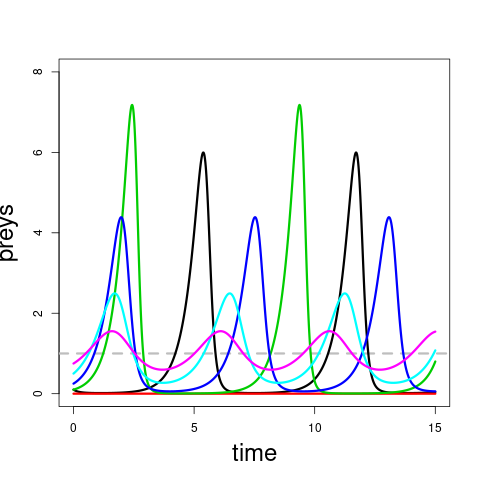
\includegraphics[width=.3\textwidth]{LotkaVolterra-preys} &
  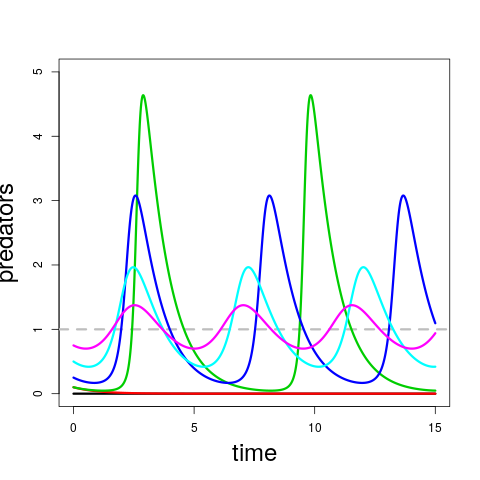
\includegraphics[width=.3\textwidth]{LotkaVolterra-predators} &
  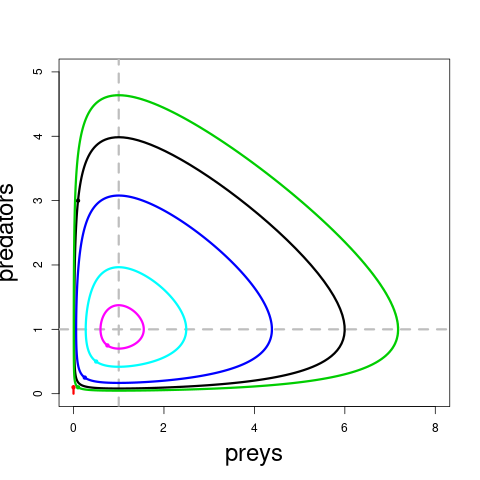
\includegraphics[width=.3\textwidth]{LotkaVolterra-preysPredators} \\
  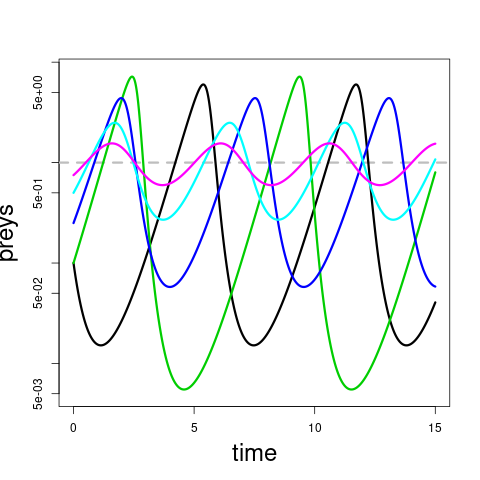
\includegraphics[width=.3\textwidth]{LotkaVolterra-preysLog} &
  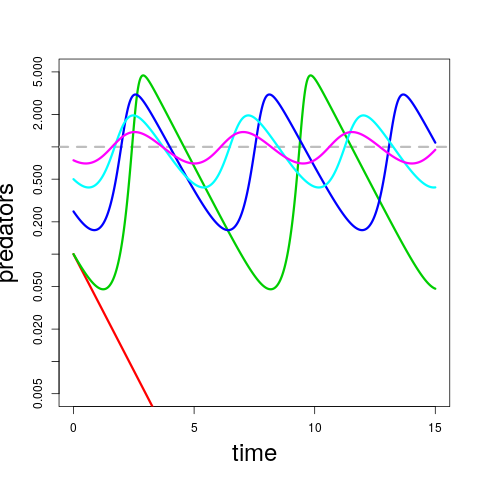
\includegraphics[width=.3\textwidth]{LotkaVolterra-predatorsLog} &
  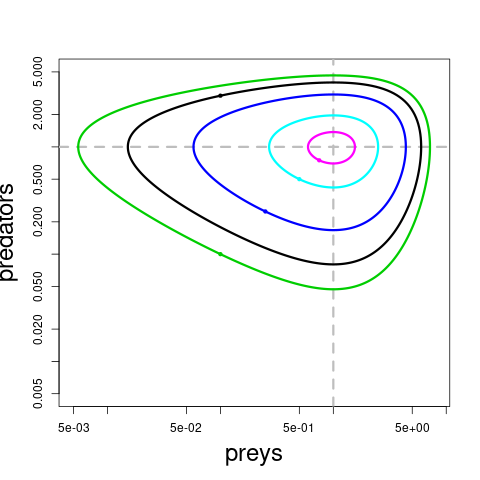
\includegraphics[width=.3\textwidth]{LotkaVolterra-preysPredatorsLog} \\
\end{tabular}
$$
}

%-------------------------------------------------------------------------------
\subsection{Modèle SIR = modèle de Kermack - McKendrick}
%-------------------------------------------------------------------------------

On rappelle le modèle pour $y(t) = [S(t) \; I(t) \; R(t)]^\top$ avec $S(t) =$ nombre de susceptibles au temps $t$, $I(t) =$ nombre d'infectés et $R(t) =$ nombre de 'remis' ({\em recovered}) :
$$
\left\{ \begin{array}{rcl} 
\dot S & = & - r S I \\
\dot I & = & r S I - a I \\
\dot R & = & a I \\
\end{array} \right.
$$
$r$ contrôle le taux d'infection et $a$ le taux de rémission.

%-------------------------------------------------------------------------------
\paragraph*{Changement de variables.}
On remarque que $\dot S + \dot I + \dot R = \dot (S + I + R) = 0$, soit 
$$
S(t) + I(t) + R(t) = \cst.
$$
On peut donc se contenter d'étudier $\{S(t), I(t), t \geq 0\}$. On peut de plus poser 
$$
x(t) = \frac{rS}a, \qquad y(t) = I,
$$
soit
$$
\left\{\begin{array}{rclcl}
        \dot x & = & -r x y & =: & F_1(x, y) \\
        \dot y & = & a y (1-x) & =: & F_2(x, y)
       \end{array}\right.
$$

\remark.
\begin{enumerate}[$a$)]
  \item $\dot x = - rxy$ est toujours négatif : la population de susceptibles décroît systématiquement ; 
  \item la croissance du nombre de susceptible $y = I$ dépend de la position de $x$ par rapport à 1 :
  $$
  \dot y \left\{\begin{array}{lll}
                < 0 & (y \downarrow) & \text{si } x > 1, \\
                = 0  & (y = \cst) & \text{si } x = 1, \\
                > 0  & (y \uparrow) & \text{si } x < 1,
                \end{array}\right..
  $$
\end{enumerate}

\dessin{Dessiner le champ de vecteurs $(\dot x, \dot y)$}

%-------------------------------------------------------------------------------
\paragraph*{Points d'équilibres.}
\begin{align*}
  F_1(x, y) & = 0 \quad \Leftrightarrow \quad x = 0 \text{ ou } y = 0 &
  \Rightarrow \qquad \Ical_1 & = \{x = 0\} \cup \{y = 0\}, \\
  F_2(x, y) & = 0 \quad \Leftrightarrow \quad y = 0 \text{ ou } x = 1 &
  \Rightarrow \qquad \Ical_2 & = \{x = 1\} \cup \{y = 0\}.
\end{align*}
Les équilibres sont donnés par l'intersection 
$$
\Ical_1 \cap \Ical_2 = \{y = 0\}
$$

%-------------------------------------------------------------------------------
\paragraph*{Nature des équilibres.}
On calcule la jacobienne
$$
J_{(x, y)}F = 
  \left[\begin{array}{ccc} 
    - r y & & -r x \\
    - a y & & a (1 - x)
  \end{array}\right].
$$
soit, pour $y = 0$
$$
J_{(x, 0)}F = 
  \left[\begin{array}{ccc} 
    0 & & -r x \\
    0 & & a (1 - x)
  \end{array}\right].
$$

%-------------------------------------------------------------------------------
\paragraph*{Nature du point d'équilibre $(x^*, 0)$.}
Le polynôme caractéristique de $J_{(x^*, 0)}F$ est
$$
P(\lambda) = \lambda (\lambda - a (1 - x^*)).
$$
Les valeurs propres sont donc $\lambda_1 = 0$ et 
$$
\lambda_2 = a (1 - x^*) 
\qquad \Rightarrow \qquad 
\left\{\begin{array}{ll} 
  \lambda_2 > 0 & \text{si } x^* < 1, \\
  \lambda_2 < 0 & \text{si } x^* > 1
\end{array} \right.
$$
et les vecteurs propres associés vérifient 
\begin{description}
  \item[pour $\lambda_1$:] 
  \begin{align*}
  \left\{\begin{array}{rcl}
      -r x^* v & = & 0 \\
      \lambda_2 v & = & 0 \\
    \end{array}\right.
    \qquad & \Rightarrow \qquad 
    v = 0 &
    \qquad & \Rightarrow \qquad 
    \left[\begin{array}{c} u=1 \\ v=0 \end{array}\right].
    \end{align*}
  \item[pour $\lambda_2$:]
    \begin{align*}
      \left\{\begin{array}{rcl}
          -r x^* v & = & \lambda_2 u \\
          \lambda_2 v & = & \lambda_2 v \\
        \end{array}\right.
        \qquad & \Rightarrow \qquad 
        v = - \frac{\lambda_2}{rx^*} u &
        \qquad & \Rightarrow \qquad 
        \left[\begin{array}{l} u=1 \\ v=-\lambda_2/(rx^*) \end{array}\right].
    \end{align*}  
\end{description}

%-------------------------------------------------------------------------------
\paragraph*{\'Etude de stabilité.}
\begin{description}
  \item[$x^* < 1$ :] dans ce cas $\lambda_2 > 0$, donc le système est instable (dans la direction verticale = infectés) : si on part avec un $y_0$ faible et un $x_0 = rS_0/a > 1$ fort, le système s'éloigne du point départ avec déclenchement d'une épidémie ($x \uparrow$)
  \item[$x^* > 1$ :] dans ce cas $\lambda_2 < 0$, donc le système est stable (dans la direction verticale = infectés) : si on part avec un $y_0$ faible et un $x_0 = rS/a < 1$ faible, le système retourne vers le un point $(x^*, 0)$ proche du point départ sans déclenchement d'une épidémie ($x \downarrow$)
\end{description}

\dessin{
$$
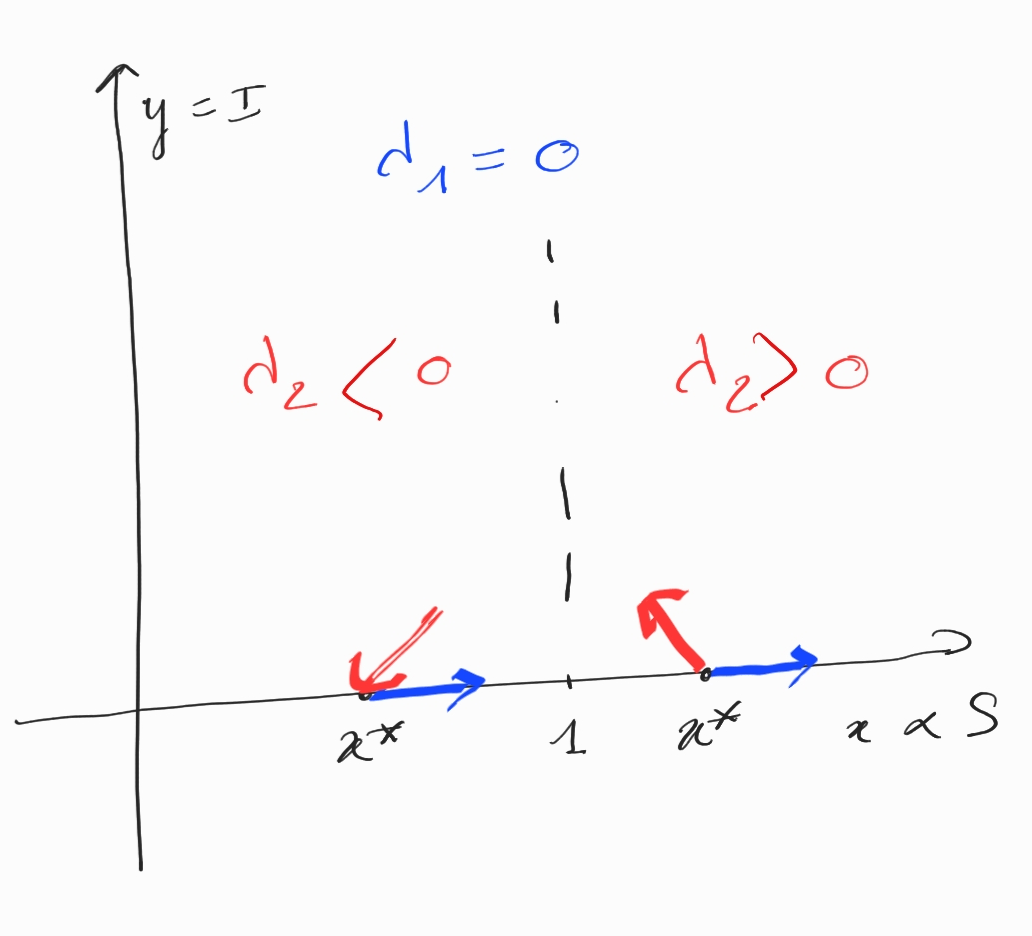
\includegraphics[width=.5\textwidth, trim=0 4 0 0, clip=]{EtudeModeleSIR}
$$
}

La trajectoire se termine toujours en un point de coordonnées $(0, x_\infty)$ avec $x_\infty < 1$, c'est à dire avec des effectifs $(S = S_\infty, I = I_\infty = 0, R_\infty = N - S_\infty)$, où $N$ est la taille constante de la population. De plus $S_\infty < a/r$ puisque $x_\infty < 1$).

\dessin{
$$
\begin{tabular}{ccc}
  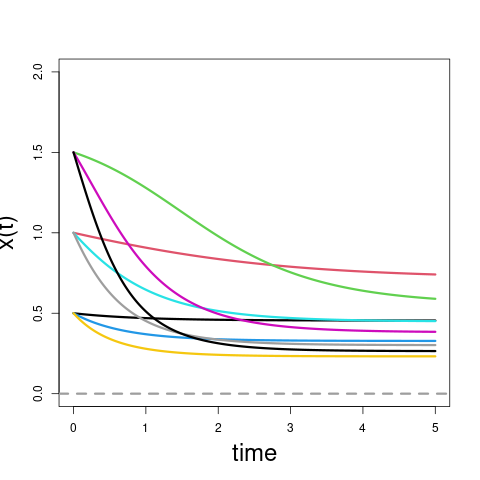
\includegraphics[width=.3\textwidth]{SIR-x} &
  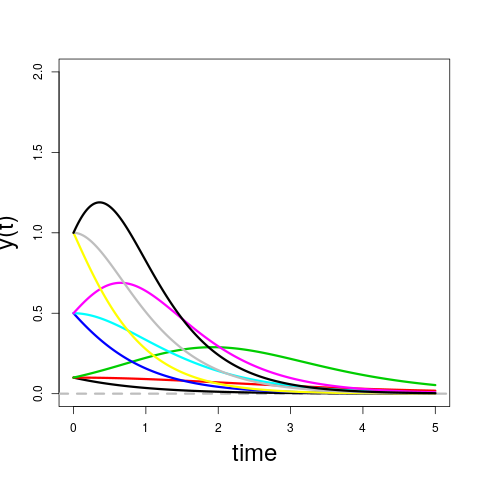
\includegraphics[width=.3\textwidth]{SIR-y} &
  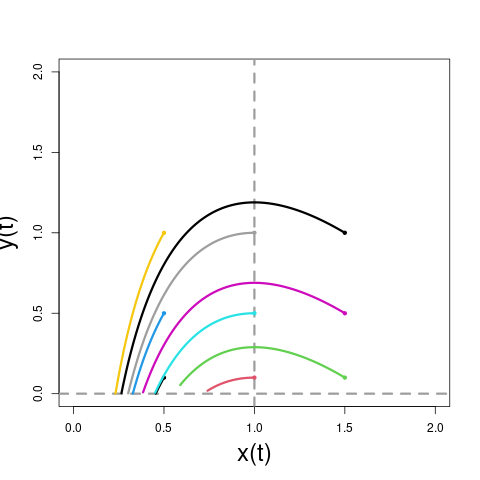
\includegraphics[width=.3\textwidth]{SIR-xy} 
\end{tabular}
$$
}

%-------------------------------------------------------------------------------
\paragraph*{Devenir de la population.}
On veut connaître les valeurs finales $(S_\infty, 0, R_\infty = N - S_\infty)$ partant d'un point $(S_0, I_0, 0)$. En reprenant la paramétrisation initiale, on remarque que, puisque
$$
\dot S = - r S I \qquad \Leftrightarrow \qquad r I = - \dot S / S,
$$
on a
$$
r \int_0^\infty I(t) \; \d t
= - \int_0^\infty \frac{\dot S(t)}{S(t)} \; \d t
= - [\log S(t)]_0^\infty
= \log \frac{S_0}{S_\infty}
$$
et que, puisque, $\dot R = aI$, on a
$$
a \int_0^\infty I(t) \; \d t
= \int_0^\infty \dot R(t) \; \d t
= [R(t)]_0^\infty
= R_\infty = N - S_\infty
$$
donc
\begin{align*}
  \frac1r \log \frac{S_0}{S_\infty} & = \frac1a (N - S_\infty) & 
  & \Leftrightarrow \qquad & 
  \log {S_0} - \log {S_\infty} & = \frac{r}a (N - S_\infty) \\
  \Leftrightarrow \qquad
  \log S_0  - N / \rho & = \log S_\infty - S_\infty / \rho &
  & \Leftrightarrow \qquad &
  S_0 e^{- N / \rho}& = S_\infty e^{- S_\infty/\rho} 
\end{align*}
pour $\rho = r/a$. On a donc
$$
f(S_\infty) = S_0 e^{- N / \rho}
\qquad \text{avec } f(x) = x e^{-x/\rho}.
$$
La fonction $f$ est nulle en 0 et $+\infty$, et sa dérivée $f'(x) = e^{-x/\rho}(1 - x/\rho)$ est positive de 0 à $\rho$, puis négative.
\dessin{
$$
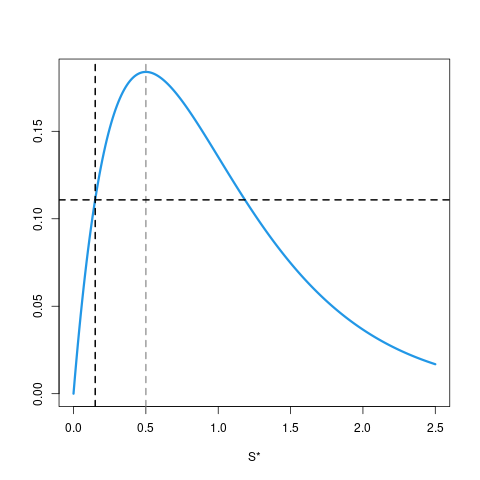
\includegraphics[width=.5\textwidth, trim=0 40 0 0, clip=]{SIR-finalState} 
$$
}
Puisqu'on sait que $x_\infty  < 1$, on a $S_\infty < \rho$ : $S_\infty$ est donné par la plus petite valeur pour laquelle $f(x)$ vaut $S_0 e^{- N / \rho}$
